% ===================================================================
\chapter{Replicating Kiem's Simulation}
\label{ch:replication}

Up to this point every comparison with Kiem has had to cross two gaps at once:
different data and a different radar. His compression ratios come from private
recordings of a single-transmitter sensor; this thesis's come from a public
twelve-transmitter cascade. Three questions could not be answered across both
gaps together:

\begin{enumerate}
\item Why did the early synthetic scenes of Section~\ref{sec:jr_synth} compress
to about 1.1 when Kiem reports 3.25?
\item Kiem says LPC is ``the same approach as DRHE'' but ``less promising''.
The LPC of this thesis is level with DRHE. Which is right?
\item Is the DRHE of this thesis the algorithm Kiem specified?
\end{enumerate}

\noindent
This chapter closes one of the gaps. It rebuilds Kiem's MATLAB simulation
\emph{from his text alone} --- his radar, his scene, his processing chain, one
transmitter --- and runs on it every coder discussed so far: DRHE with and
without run-length coding, with his fixed dictionary and with an ideal one; the
LPC-Huffman of his reference \cite{meucci2022}; the slow-time LPC of this thesis; no
prediction; and approximations of his lossy schemes. The third question is
answered in Chapter~\ref{ch:kiemcompare}, using a cross-check made here.

\section{What was built}
\label{sec:kr_built}

The replication lives in \texttt{ThesisA/kiem\_replication} and is
deliberately independent: it uses base MATLAB only and calls nothing in
\texttt{Matlab\_Sim}. Its stages follow Kiem's Figure~3.1 and are listed in
Table~\ref{tab:kr_files} with the section of his thesis each one implements.

\begin{table}[htbp]
\centering
\caption[Replication: stages and sources]{The replication, stage by stage,
with the part of Kiem's thesis each stage is built from.}
\label{tab:kr_files}
\small
\begin{tabular}{@{}p{42mm}p{62mm}p{28mm}@{}}
\toprule
File & Role & Kiem\\
\midrule
\texttt{kr\_config.m} & every parameter, with its source or ``ASSUMPTION'' & Tables 3.2, 3.3, 4.4; App.\ A\\
\texttt{kr\_generate\_adc.m} & beat signals of the targets, AWGN, 14-bit ADC; optional TDM interleaving & \S{}3.2.2\\
\texttt{kr\_calibrate\_noise.m} & ADC noise level that gives a chosen noise floor after NCI & Table 3.2\\
\texttt{kr\_preprocess\_fft.m} & shift to 32-bit full scale, Hanning, FFT$/N$, first half & \S{}3.2.1, \S{}4.3.3\\
\texttt{kr\_fp16.m}, \texttt{kr\_fx16.m} & FP16 reference; FX16 in two scalings & \S{}3.4.1\\
\texttt{kr\_second\_stage.m}, \texttt{kr\_detect.m} & Doppler FFT, NCI, noise threshold and local maxima & \S{}3.2.1\\
\texttt{kr\_metrics.m} & CR, FN\%, FP\%, NF, SNR against FP16 & \S{}3.4.2\\
\texttt{kr\_drhe\_*.m} & DRHE model prediction and its inverse & \S{}3.5.3, \S{}3.5.4\\
\texttt{kr\_bits\_s4.m}, \texttt{kr\_bits\_r4s4.m} & S4 coder (fixed or ideal dictionary); original R4S4 + RLE coder & Table 3.7, \S{}2.7.3, \S{}3.5.1\\
\texttt{kr\_lpc\_raw.m} & LPC-Huffman of \cite{meucci2022}: fast-time prediction of raw ADC & \S{}2.7.4\\
\texttt{kr\_lpc\_fft.m} & this thesis's slow-time LPC, for comparison & ---\\
\texttt{kr\_lossy.m} & approximations of CMPRA/B and EGE10/8/6/4 & \S{}2.7.1, \S{}2.7.2\\
\texttt{run\_kiem\_replication.m} & the whole workflow at two noise levels & Fig.\ 3.1\\
\bottomrule
\end{tabular}
\end{table}

\noindent
Every lossless path is decoded and compared with its input on every run; none
is assumed lossless. Building the DRHE decoder exposed one subtlety worth
recording. MATLAB's \texttt{round} returns $-0$ for small negative values, and
$\mathrm{atan2}(-0, x<0) = -\pi$ while $\mathrm{atan2}(+0, x<0) = +\pi$. The
encoder saw $-0$ and the decoder, which rebuilds the value as an integer, saw
$+0$; their phase predictions differed by $2\pi$ and the round trip failed. The
FX16 quantiser now normalises $-0$ to $+0$. A hardware implementation never
meets this, because integers have no negative zero, but a floating-point model
of one can.

\subsection{The radar and the scene}

The radar is Kiem's Table~3.2: one MMIC, \textbf{one transmitter}, four
receivers, 1024 samples per ramp, 512 ramps, a 14-bit ADC. The scene has his
five targets at range bins [100, 150, 150, 200, 400] and Doppler bins [50, 50,
100, 200, 250] with amplitudes [0.8, 0.3, 0.4, 0.5, 0.7] of full scale, and
white Gaussian noise set so that the noise floor after NCI is his
$-75$\,dBFS. Figure~\ref{fig:kr_scene} shows it; it is visibly the scene of his
Figures~3.5 and~3.7.

\begin{figure}[htbp]
\centering
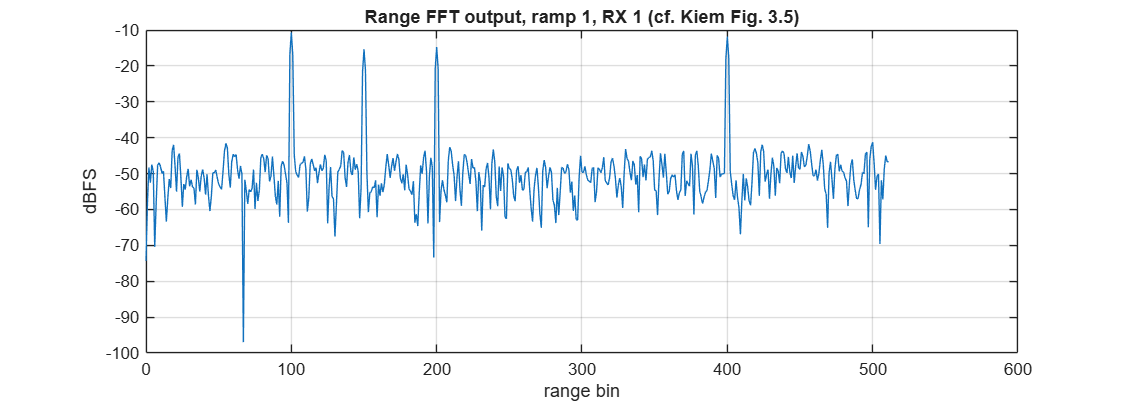
\includegraphics[width=0.49\textwidth]{fig_kr_rangefft.png}\hfill
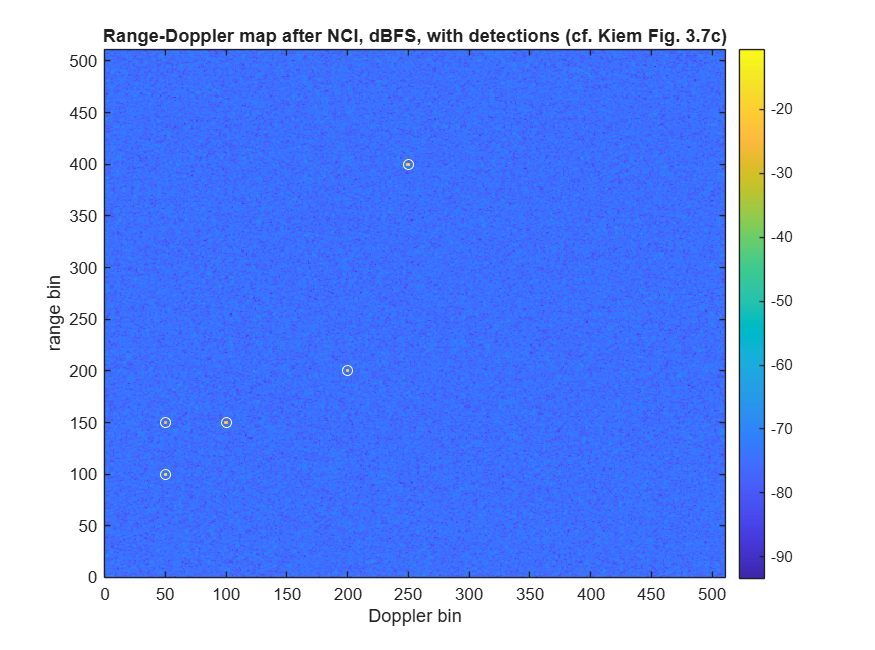
\includegraphics[width=0.46\textwidth]{fig_kr_rdmap.png}
\caption[The replicated scene]{Kiem's Table~3.2 scene as rebuilt. Left: range
FFT of ramp 1, receiver 1 (compare his Figure~3.5). Right: range--Doppler map
after NCI with the five reference detections circled (compare his
Figure~3.7c).}
\label{fig:kr_scene}
\end{figure}

\subsection{Where Kiem's text leaves a choice}
\label{sec:kr_assump}

Seven parameters are not given in his thesis. Each is set in one place
(\texttt{kr\_config.m}), marked there as an assumption, and can be changed.

\begin{description}[leftmargin=!,labelwidth=30mm,style=nextline,font=\normalfont\bfseries]
\item[Target angles] Not given. Fixed, distinct angles
($-30^\circ$, $-10^\circ$, $0^\circ$, $15^\circ$, $40^\circ$) on a
half-wavelength array, so the four receive channels differ.
\item[Amplitudes] His five amplitudes sum to 2.7 of full scale, which a 14-bit
ADC cannot hold without clipping. They are scaled together so the worst-case
sum just fits.
\item[FX16 scaling] Two modes: \emph{hw}, the top 16 bits of the 32-bit FFT
word, which is what his FFT core delivers (default); and \emph{peak}, the
Matlab\_Sim scaling in which a full-scale sinusoid maps to 32767. They differ by
exactly a factor of four.
\item[0\,dBFS] Not defined in his thesis. The NCI power of a full-scale
sinusoid through the whole chain (as in Matlab\_Sim) is the default; the power
of a unit value in the 32-bit word is also reported, and reads 12.0\,dB lower.
\item[Detector] Noise estimate the mean dB of the lowest \SI{75}{\percent} of
cells; threshold 15\,dB above it; 8-neighbour local maxima.
\item[Noise floor and SNR] The noise floor is the mean dB outside a
$5\times5$ patch around each detection; SNR is the RMS peak power in dB minus it,
as in his Section~3.4.2.
\item[LPC-Huffman of Meucci and Mancuso] Order not given, so $p = 1 \ldots 10$ is swept;
one coefficient set per chirp and receiver, sent as 32-bit floats; the
Huffman dictionary counted at 21 bits per symbol used.
\end{description}

\noindent
His lossy schemes cannot be reproduced exactly, because their bit layouts are
proprietary. They are approximated --- CMPRA and CMPRB as block floating point
with one 4-bit exponent per 256-bit word, EGE-$k$ as blocks of eight complex
bins with an 8-bit header and least significant bits dropped to meet CR
$16/k$ --- and are included for completeness rather than as evidence.

\section{Results at Kiem's noise level}
\label{sec:kr_m75}

Table~\ref{tab:kr_m75} runs the complete workflow at the $-75$\,dBFS of his
Table~3.2 and sets his published Table~3.5 beside it. The published numbers are
from his real recordings, not from this scene; they are there to be read
against, not matched.

\begin{table}[htbp]
\centering
\caption[Replication at $-75$\,dBFS]{Kiem's workflow on his Table~3.2 scene at
his $-75$\,dBFS noise floor (\texttt{results/run\_kiem\_replication\_log.txt}),
beside his Table~3.5. ADC noise $\sigma = 375.9$ codes; FX16 noise
\num{20.35}\,LSB; five reference detections. ``(approx.)'' marks schemes
approximated because their exact layout is proprietary.}
\label{tab:kr_m75}
\small
\setlength{\tabcolsep}{4pt}
\begin{tabular}{@{}lrrrrr@{\hskip 12pt}rrr@{}}
\toprule
& \multicolumn{5}{c}{\textbf{replication}} & \multicolumn{3}{c}{\textbf{Kiem, real data}}\\
\cmidrule(lr){2-6}\cmidrule(lr){7-9}
Algorithm & CR & FN\% & FP\% & NF & SNR & CR & FN\% & FP\%\\
\midrule
FP16 (reference)                   & 1.00 & 0 & 0 & $-75.00$ & 61.50 & 1.00 & 0 & 0\\
FX16                               & 1.00 & 0 & 0 & $-75.00$ & 61.50 & 1.00 & 0.59 & 1.18\\
CMPRA (approx.)                    & 2.00 & 0 & 0 & $-74.86$ & 61.36 & 2.00 & 0.59 & 0.59\\
CMPRB (approx.)                    & 4.00 & 0 & 13980 & $-75.56$ & 40.55 & 4.00 & 7.69 & 4.73\\
EGE10 (approx.)                    & 1.60 & 0 & 0 & $-75.00$ & 61.50 & 1.60 & 1.18 & 1.18\\
EGE8 (approx.)                     & 2.00 & 0 & 0 & $-74.98$ & 61.48 & 2.00 & 2.37 & 2.37\\
EGE6 (approx.)                     & 2.67 & 0 & 0 & $-74.79$ & 61.29 & 2.67 & 7.69 & 7.10\\
EGE4 (approx.)                     & 4.00 & 0 & 680 & $-74.71$ & 52.31 & 4.00 & 40.24 & 26.63\\
\textbf{DRHE, R4S4 + RLE}          & \textbf{2.28} & 0 & 0 & $-75.00$ & 61.50 & \textbf{3.25} & 0.59 & 1.18\\
DRHE, S4 only, ideal dictionary    & 2.28 & 0 & 0 & $-75.00$ & 61.50 & 3.24 & 0.59 & 1.18\\
DRHE, S4, Kiem's fixed dictionary  & 1.85 & 0 & 0 & $-75.00$ & 61.50 & (3.17 HW) & & \\
LPC-Huffman, raw ADC \cite{meucci2022}, $p=10$  & 1.32 & 0 & 0 & $-75.00$ & 61.50 & (2.056 in \cite{meucci2022}) & & \\
LPC, slow time (this thesis)       & 2.06 & 0 & 0 & $-75.00$ & 61.50 & & & \\
No prediction, fixed dictionary    & 2.03 & 0 & 0 & $-75.00$ & 61.50 & & & \\
\bottomrule
\end{tabular}
\end{table}

\noindent
Three things stand out.

\paragraph{DRHE compresses to 2.28 on Kiem's own scene, not 3.25.} The scene
is his, the chain is his and the algorithm is his (Section~\ref{sec:kc_audit}
shows it is exactly his). The ratio is not.

\paragraph{The detection columns do not resemble his.} This scene has five
targets 60 to 74\,dB above the noise; his recordings had about 170 detections
at 22\,dB. With five detections, one miss would be \SI{20}{\percent}, so FN and
FP are not comparable at all. The same high SNR is why the approximated lossy
schemes produce large false-discovery rates here: at 60\,dB SNR a 3-bit mantissa
leaves quantisation spurs in the range--Doppler map that are 20 to 40\,dB above
the noise and are detected as targets. Those FP percentages describe this scene,
not the schemes.

\paragraph{Prediction is doing almost nothing.} No prediction at all gives 2.03
through the fixed dictionary; DRHE gives 1.85 and the slow-time LPC 2.06. In a
scene that is 99.99\,\% noise cells there is nothing to predict: noise at ramp
$m-1$ says nothing about noise at ramp $m$. Section~\ref{sec:kr_sweep}
shows this holds at every noise level.

\section{The noise level at which DRHE gives 3.25}
\label{sec:kr_m88}

On a white-noise scene the compression ratio depends on one thing above all:
the standard deviation of the noise in FX16 least significant bits. A bisection
on the noise floor (\texttt{kr\_find\_nf\_for\_cr.m}) finds the level at which
DRHE with run-length coding gives Kiem's 3.25: $-87.9$\,dBFS, where the ADC
noise is 85.4 codes and the FX16 noise 4.63\,LSB. Table~\ref{tab:kr_m88} gives
the full workflow there.

\begin{table}[htbp]
\centering
\caption[Replication at $-87.9$\,dBFS]{The same workflow at the noise floor
where DRHE reproduces Kiem's 3.25 (\texttt{run\_kiem\_replication\_log.txt},
operating point 2). ADC noise $\sigma = 85.4$ codes; FX16 noise 4.63\,LSB.
Detection metrics are omitted: every lossless row equals FX16's (0/0).}
\label{tab:kr_m88}
\small
\begin{tabular}{@{}lrr@{}}
\toprule
Coder & replication & Kiem\\
\midrule
DRHE, R4S4 + RLE, ideal Huffman     & \textbf{3.25} & \textbf{3.25} (Table 3.5)\\
DRHE, S4 only, ideal Huffman        & \textbf{3.24} & \textbf{3.24} (Table 3.6)\\
DRHE, S4, Kiem's fixed dictionary   & 3.23 & 3.17 (hardware, different FFT)\\
LPC-Huffman on raw ADC \cite{meucci2022}, $p=10$ & 1.54 & not run (2.056 in \cite{meucci2022})\\
LPC, slow time, fixed dictionary    & 3.38 & ---\\
LPC, slow time, ideal Huffman       & 3.43 & ---\\
No prediction, fixed dictionary     & 3.26 & ---\\
No prediction, R4S4 + RLE           & 3.38 & ---\\
\bottomrule
\end{tabular}
\end{table}

\noindent
At this one noise level the replication reproduces Kiem's DRHE pattern
exactly: 3.25 with run-length coding, 3.24 without (his Table~3.6), and almost
no loss from fixing the dictionary (3.23). It reproduces his observation that
run-length coding adds nearly nothing. But the operating point was
\emph{chosen} to give 3.25; it is not a prediction. And it sits
\SI{17.2}{\decibel} below the $-70.7$\,dBFS noise floor he reports with that
3.25.

\section{Compression ratio across noise levels}
\label{sec:kr_sweep}

Figure~\ref{fig:kr_sweep} sweeps the noise floor from $-120$ to $-60$\,dBFS
on the same scene (\texttt{kr\_noise\_sweep.m}), for both FX16 scalings, and
places on it the early Matlab\_Sim scenes of Table~\ref{tab:jr_synth} and
Kiem's published result.

\begin{figure}[htbp]
\centering
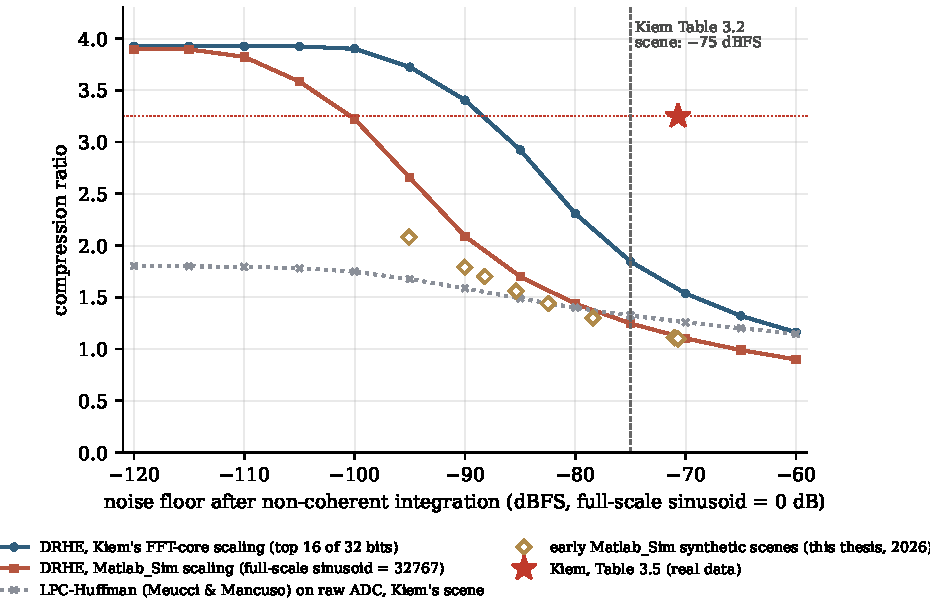
\includegraphics[width=\textwidth]{fig_kr_sweep.pdf}
\caption[CR against noise floor on Kiem's scene]{Compression ratio against
noise floor on Kiem's Table~3.2 scene with one transmitter. Blue: DRHE with
Kiem's fixed dictionary and his FFT core's scaling. Red: the same with the
Matlab\_Sim scaling, four times larger. Grey: LPC-Huffman of \cite{meucci2022} on raw ADC.
Diamonds: the early synthetic scenes of this thesis. Star: Kiem's published
3.25 at $-70.7$\,dBFS, which lies 17\,dB to the right of where his own
scaling's curve passes 3.25.}
\label{fig:kr_sweep}
\end{figure}

The curves have three regimes.

\begin{itemize}
\item \textbf{Very low noise} (left). The FX16 noise rounds to zero, the
residuals are nearly all zero, and the fixed dictionary's floor takes over:
every value costs at least four bits (Section~\ref{sec:huffman}), so the ratio
saturates just below 4.0 (3.92). With run-length coding and an ideal dictionary
it would grow without limit (82 at $-140$\,dBFS), because long runs of zeros
cost almost nothing; that regime is irrelevant to a real radar.
\item \textbf{The transition} (centre). Each 6\,dB of extra noise doubles the
noise in LSB, adds about one bit to every residual and lowers the ratio.
\item \textbf{High noise} (right). Every value carries several bits of noise
and the ratio falls towards 1.
\end{itemize}

\noindent
The two scalings produce the same curve shifted by 12\,dB, as a factor of four
in amplitude must. Along both curves, no prediction and the slow-time LPC stay
within about ten per cent of DRHE either way, and with the fixed dictionary no
prediction is often the better of the two (Table~\ref{tab:kr_m75},
Table~\ref{tab:kr_m88} and \texttt{noise\_sweep.csv}): on white noise the
predictor is not what sets the ratio.

\section{Why the early simulations gave 1.1}
\label{sec:kr_early}

Table~\ref{tab:kr_early} (\texttt{kr\_early\_result\_check.m}) runs Kiem's
scene at three noise floors with both scalings.

\begin{table}[htbp]
\centering
\caption[FX16 scaling and noise floor]{DRHE and the other coders on Kiem's
scene for both FX16 scalings (\texttt{results/early\_result\_check.txt}).
``Noise'' is the standard deviation of FX16 codes in noise-only range bins.}
\label{tab:kr_early}
\small
\begin{tabular}{@{}lrrrrrr@{}}
\toprule
FX16 scaling & NF (dBFS) & noise (LSB) & DRHE, fixed & DRHE, R4S4 & LPC & no pred.\\
\midrule
hw (Kiem's FFT core) & $-70.7$ & 33.4 & 1.57 & 2.07 & 1.73 & 1.71\\
hw                   & $-75.0$ & 20.4 & 1.85 & 2.28 & 2.06 & 2.03\\
hw                   & $-87.9$ & 4.6  & \textbf{3.24} & 3.25 & 3.38 & 3.26\\
peak (Matlab\_Sim)   & $-70.7$ & 133.4 & \textbf{1.12} & 1.64 & 1.20 & 1.19\\
peak                 & $-75.0$ & 81.3 & 1.25 & 1.78 & 1.34 & 1.32\\
peak                 & $-87.9$ & 18.4 & 1.91 & 2.32 & 2.13 & 2.08\\
\bottomrule
\end{tabular}
\end{table}

\noindent
The row ``peak, $-70.7$\,dBFS'' gives 1.12. That is the early Matlab\_Sim
result (1.10--1.12, Table~\ref{tab:jr_synth}) reproduced in an independent code
base from nothing but Kiem's text and the Matlab\_Sim scaling. Two factors
multiply to produce it:

\begin{itemize}
\item \textbf{The scaling, a factor of four.} Matlab\_Sim maps a full-scale
sinusoid to 32767; Kiem's core keeps the top 16 bits of the 32-bit word, where
it is about 8191. The same noise therefore occupies four times as many LSB,
about two more bits per value.
\item \textbf{The noise floor, a factor of seven.} Matching Kiem's stated
$-70.7$\,dBFS with white noise gives 33\,LSB even with his scaling; his CR of
3.25 needs about 4.6\,LSB.
\end{itemize}

\noindent
Together: 133\,LSB of noise where his result implies about 5, some thirty times
more. The early explanation --- that white noise lacks the slow-time
correlation DRHE needs --- was right that white noise is unpredictable, but
wrong that this was what set the ratio: the no-prediction column shows the same
ratios without any predictor.

\section{Kiem's noise floor and his compression ratio do not agree}
\label{sec:kr_nfcr}

The replication cannot make Kiem's reported noise floor and his reported
compression ratio hold together on a white-noise scene, under any reading of
his text. With his FFT scaling, CR 3.25 needs $-87.9$\,dBFS by the
full-scale-sinusoid reference or $-99.9$\,dBFS by the unit reference; he
reports $-70.7$\,dBFS. These are the only two references his text suggests, and
the second only widens the gap.

\subsection{His dictionary says what his residuals looked like}
\label{sec:kr_fingerprint}

Kiem built his fixed Huffman dictionary from the S4 statistics of his own
residuals (Section~\ref{sec:kiem_adapt}). A Huffman code is optimal only for
the distribution it was built from, so its lengths can be read backwards.
Table~\ref{tab:kr_fp} (\texttt{kr\_dictionary\_fingerprint.m}) codes
integer-rounded Gaussian residuals of increasing spread with his dictionary and
with the ideal code for each spread.

\begin{table}[htbp]
\centering
\caption[What Kiem's dictionary was built for]{Kiem's fixed dictionary
against an ideal Huffman code on Gaussian residuals
(\texttt{results/dictionary\_fingerprint.txt}). The overhead is smallest where
the dictionary matches the data it was made from.}
\label{tab:kr_fp}
\small
\begin{tabular}{@{}rrrrr@{}}
\toprule
Residual std (LSB) & CR, Kiem's dictionary & CR, ideal code & overhead & commonest S4\\
\midrule
1   & 4.00 & 6.80 & \SI{70.1}{\percent} & 1\\
2   & 3.92 & 4.84 & \SI{23.2}{\percent} & 2\\
4   & 3.60 & 3.75 & \SI{4.1}{\percent}  & 2\\
5   & 3.46 & 3.48 & \SI{0.6}{\percent}  & 3\\
\textbf{6}   & \textbf{3.33} & \textbf{3.33} & \textbf{\SI{0.0}{\percent}}  & 3\\
\textbf{7}   & \textbf{3.20} & \textbf{3.20} & \textbf{\SI{0.0}{\percent}}  & 3\\
\textbf{8}   & \textbf{3.07} & \textbf{3.07} & \textbf{\SI{0.1}{\percent}}  & 3\\
10  & 2.82 & 2.88 & \SI{2.2}{\percent}  & 4\\
15  & 2.38 & 2.63 & \SI{10.2}{\percent} & 4\\
20  & 2.12 & 2.45 & \SI{15.8}{\percent} & 5\\
33  & 1.76 & 2.21 & \SI{25.6}{\percent} & 5\\
\bottomrule
\end{tabular}
\end{table}

\noindent
The dictionary is optimal for residuals with a standard deviation of 6 to
8\,LSB and costs \SI{26}{\percent} for the 33\,LSB that his reported noise floor
would give on white noise. Its fingerprint agrees with his CR of 3.25 and with
his residual histograms (his Figures~3.9--3.10, ``most values'' within
$\pm 40$); it does not agree with a white-noise floor at $-70.7$\,dBFS.

\subsection{The most likely reconciliation}

His Table~3.5 was measured on real recordings. In real data the ``mean of the
noisy part of the signal in dB'' can be raised by clutter, leakage, sidelobes
and slowly varying returns in the cells the estimator averages, while most cells
--- which set the compression ratio --- sit much lower. In a white-noise
simulation the noise floor and the per-cell noise are the same number, so
matching his noise floor forces far too much noise into every cell. This
reconciliation fits every figure available: his ratio, his dictionary and his
histograms. It cannot be confirmed without his data or code, and it is reported
as an inference, not a finding.

\section{LPC-Huffman, the method Kiem excluded}
\label{sec:kr_lpcraw}

\texttt{kr\_lpc\_raw.m} implements LPC-Huffman as Kiem describes it: a $p$-th
order predictor of each raw ADC sample from the previous $p$ samples of the same
chirp, Levinson--Durbin coefficients per chirp and receiver, sent as 32-bit
floats, and a Huffman code built from the residuals. The decoder runs sample by
sample and the round trip is checked.

\begin{table}[htbp]
\centering
\caption[LPC-Huffman of Meucci and Mancuso by order]{LPC-Huffman on the raw ADC samples of
Kiem's scene, by predictor order (\texttt{run\_kiem\_replication\_log.txt}; CR
including the dictionary). Five real sinusoids need up to ten poles.}
\label{tab:kr_lpcorder}
\small
\begin{tabular}{@{}rrrrr@{}}
\toprule
& \multicolumn{2}{c}{$-75$\,dBFS} & \multicolumn{2}{c}{$-87.9$\,dBFS}\\
\cmidrule(lr){2-3}\cmidrule(lr){4-5}
$p$ & CR & residual std (codes) & CR & residual std (codes)\\
\midrule
1  & 1.174 & 2686 & 1.176 & 2660\\
2  & 1.172 & 2682 & 1.174 & 2655\\
4  & 1.204 & 2014 & 1.208 & 1966\\
6  & 1.312 & 921  & 1.388 & 602\\
8  & 1.310 & 899  & 1.426 & 506\\
10 & \textbf{1.324} & 799 & \textbf{1.543} & 318\\
\bottomrule
\end{tabular}
\end{table}

\noindent
On Kiem's own scene, at either noise level, the method he excluded loses to
DRHE by a wide margin (1.32 against 1.85--2.28; 1.54 against 3.23--3.25), and
it stays below 1.8 across the whole sweep (Figure~\ref{fig:kr_sweep}).
\textbf{For the LPC he meant, Kiem's ranking holds.} It holds for a reason that
has little to do with the predictor.

\paragraph{Raw-ADC coding must keep bits the FX16 step has already discarded.}
Kiem's chain shifts the 14-bit samples left by 18 bits, windows them, takes the
FFT divided by $N$ and keeps the top 16 bits. White ADC noise of standard
deviation $\sigma$ codes therefore reaches the FX16 word with standard
deviation
\begin{equation}
\label{eq:noisemap}
\sigma_{\mathrm{FX16}} = \sigma \cdot \frac{2^{18}}{2^{16}} \cdot
\frac{\sqrt{\sum_k w_k^2 / 2}}{N}
= \sigma \cdot 4 \cdot \sqrt{\frac{0.375}{2 \times 1024}} = 0.0541\,\sigma,
\end{equation}
using $\sum_k w_k^2 \approx 0.375N$ for a Hanning window. The simulation
measures exactly this ratio: 375.9 codes become 20.35\,LSB and 85.4 codes become
4.63\,LSB. The FFT scaling and the truncation to 16 bits thus discard
$\log_2(1/0.0541) \approx 4.2$ bits of noise per value before DRHE ever sees the
data. A lossless coder of the raw samples must keep them. At $-87.9$\,dBFS even a
perfect predictor would leave a residual of at least the ADC noise, 85 codes,
whose entropy is about $\log_2(85\sqrt{2\pi e}) \approx 8.5$ bits, capping the
ratio near $16/8.5 \approx 1.9$; the prediction filter then amplifies white
noise, and the measured ratio is 1.54.

So the comparison Kiem made on paper is between a lossless coder of the ADC
stream and a lossless coder of already-truncated data. The truncation is the
lossy step, and his Table~3.5 shows its cost in the FX16 row
(\SI{0.59}{\percent} missed, \SI{1.18}{\percent} spurious). DRHE inherits that
cost; LPC-Huffman on raw ADC does not.

\paragraph{The coefficient method is not the problem.} The Levinson--Durbin
(autocorrelation) method is biased for pure sinusoids over a finite record; the
covariance (true least-squares) method is not. Replacing one with the other
(\texttt{kr\_lpc\_raw\_method\_check.m}) raises the ratio only when there is
almost no noise --- from 1.83 to 6.51 at $-140$\,dBFS, $p = 10$ --- and changes
nothing at the noise levels that matter: 1.56 against 1.59 at $-87.9$\,dBFS and
1.34 against 1.34 at $-75$\,dBFS.

\paragraph{The slow-time LPC is a different matter.} On the same scene the LPC
of this thesis --- same domain and coder as DRHE --- gives 2.06 against DRHE's
1.85 at $-75$\,dBFS and 3.38 against 3.23 at $-87.9$\,dBFS, and it stays level
with or slightly above DRHE across the sweep from $-95$\,dBFS upwards. On
Kiem's scene, the controlled comparison comes out the other way from his
remark.

\section{Adding transmitters}
\label{sec:kr_tdm}

The replication can also do what Kiem's radar cannot: interleave the ramps
over twelve transmitters, each at its own position in a virtual array, as in
the ColoRadar cascade (\texttt{kr\_tdm\_experiment.m}). Two scenes are used:
Kiem's five-target scene, and a denser one that is \emph{not} from Kiem --- 300
slowly moving scatterers between $-70$ and $-30$\,dB of full scale at random
angles, a stand-in for a real indoor scene.

\begin{table}[htbp]
\centering
\caption[One against twelve transmitters]{DRHE (fixed dictionary) and the other
coders with one transmitter and with twelve interleaved, predicting from the
previous ramp (lag 1) or from the previous ramp of the same transmitter
(lag 12). \texttt{results/tdm\_experiment.txt}.}
\label{tab:kr_tdm}
\small
\begin{tabular}{@{}llrrrr@{}}
\toprule
Scene, noise floor & radar, lag & DRHE & DRHE+RLE & LPC & no pred.\\
\midrule
Kiem, $-75$\,dBFS  & 1 TX, lag 1   & 1.850 & 2.285 & 2.070 & 2.036\\
                   & 12 TX, lag 1  & 1.836 & 2.262 & 2.051 & 2.036\\
                   & 12 TX, lag 12 & 1.859 & 2.283 & 2.056 & 2.036\\
\midrule
Kiem, $-95$\,dBFS  & 1 TX, lag 1   & 3.726 & 4.237 & 3.760 & 3.603\\
                   & 12 TX, lag 1  & 3.641 & 4.120 & 3.666 & 3.603\\
                   & 12 TX, lag 12 & 3.694 & 4.208 & 3.665 & 3.603\\
\midrule
Dense, $-75$\,dBFS & 1 TX, lag 1   & 1.772 & 2.203 & 1.960 & 1.656\\
                   & 12 TX, lag 1  & 1.647 & 2.066 & 1.798 & 1.657\\
                   & 12 TX, lag 12 & 1.689 & 2.110 & 1.840 & 1.657\\
\midrule
Dense, $-95$\,dBFS & 1 TX, lag 1   & \textbf{3.398} & 3.516 & 3.596 & 1.952\\
                   & 12 TX, lag 1  & \textbf{2.371} & 2.514 & 2.462 & 1.955\\
                   & 12 TX, lag 12 & \textbf{2.560} & 2.673 & 2.712 & 1.955\\
\bottomrule
\end{tabular}
\end{table}

\noindent
On Kiem's scene the transmitters make almost no difference, because there is
almost nothing but noise to predict. On the dense scene at low noise, prediction
earns its keep --- DRHE 3.40 against 1.95 without prediction --- and TDM
interleaving costs it a third of its ratio (2.37). Predicting from the same
transmitter recovers part of the loss (2.56). The recovery is only partial here;
the likely reasons are that each transmitter's predictor starts from zero, so
there are twelve cold starts per frame instead of one, and that the synthetic
scatterers move, so each lag-12 prediction spans a Doppler step twelve times
larger than a lag-1 prediction on a single-transmitter radar. This is the mechanism of Section~\ref{sec:predaxisresults}, reproduced in
a scene built from Kiem's parameters.

\section{Is the DRHE here the DRHE there?}
\label{sec:kr_crosscheck}

\texttt{kr\_crosscheck\_matlabsim.m} --- the one file of the replication that
touches Matlab\_Sim, and only to verify it --- runs the thesis's
\texttt{compress\_drhe.m} and the replication's DRHE, written independently from
Kiem's Section~3.5.3, on the same FX16 frames. They produce \emph{identical}
residuals and identical bit counts: \num{18186374} bits at $-75$\,dBFS and
\num{10370342} at $-87.9$\,dBFS, a difference of zero in each. The HLS DRHE-1
reproduces \texttt{compress\_drhe.m}'s bit counts on all 50 ColoRadar frames
(Section~\ref{sec:phase2}), and an independent Python implementation reproduces
the HLS bit counts exactly (Appendix~\ref{app:verify}). The chain from Kiem's
specification to the hardware is therefore closed at every link.
Section~\ref{sec:kc_audit} goes through the specification line by line.

\section{What the replication shows, and what it cannot}
\label{sec:kr_limits}

\begin{keybox}
\textbf{It shows} that Kiem's workflow, rebuilt from his text, reproduces his
DRHE pattern (3.25 with run-length coding, 3.24 without, almost nothing lost
to the fixed dictionary) at one noise level; that the early 1.1 of this project
is explained completely by the FX16 scaling and the noise floor; that the
LPC-Huffman he excluded does lose to DRHE, mainly because it codes raw ADC noise
that the FX16 step discards; that the slow-time LPC of this thesis does not lose;
and that the DRHE of this thesis is his algorithm, to the bit.

\textbf{It cannot} reproduce his absolute numbers, which come from recordings
that are not available, and the operating point that matches his CR is chosen,
not predicted. The reconciliation of his noise floor with his ratio is an
inference. His lossy schemes are approximations, and the detection metrics of
a five-target scene say nothing about a 170-detection one.
\end{keybox}
